\documentclass[12pt]{article}
\usepackage{amsmath,amssymb,amsthm,epsf, graphics, rotating}
\usepackage{tikz}

\pagestyle{empty}
\setlength{\parindent}{0pt}
\setlength{\textwidth}{6.5in}
\setlength{\oddsidemargin}{0in}
\addtolength{\textheight}{1in}

\renewcommand\theenumi{\alph{enumi}}
\renewcommand\labelenumi{(\theenumi)}


\newcommand{\Z}{\mathbb{Z}}
\newcommand{\F}{\mathbb{F}}
\newcommand{\R}{\mathbb{R}}
\newcommand{\C}{\mathbb{C}}
\renewcommand\vec{\mathbf}

\theoremstyle{definition}
\newtheorem{problem}{}
\newtheorem{solution}{}
\title{\vspace{-2.0cm}Math 442 Homework 3}
\date{}

%\renewcommand{\bigskip}{\vfill}

\begin{document}
%\vspace*{-1.2in}
%
%
\maketitle
%
\vspace{-16 mm}
\begin{itemize}
\item Due Thursday January 24th at start of class.
%
\item If your homework is longer than one page, {\bf staple} the pages together, and put your name on each sheet of paper.
%
\item {\bf Collaboration Policy}: You are welcome (and encouraged) to work on the homework in groups. However, each student must write up the homework on their own, and must use their own wording (i.e.~don't jusy copy the solutions from your friend). If you do collaborate with others, please list the name of your collaborators at the top of the homework.

\item You are encouraged (though not required) to type up your solutions. If you choose to do this, I strongly recommend that you use the typesetting software LaTeX. LaTeX is used by the entire mathematics community, and if you intend to go into math, you’ll need to learn it sooner or later. ``The Not So Short Introduction to LaTeX'' is a good place to start. This guide can be found at http://tug.ctan.org/info/lshort/english/lshort.pdf . You can also download the .tex source file for this homework and take a look at that.

\item Each homework problem should be correct as stated. Occasionally, however, I might screw something up and give you an impossible homework problem. If you believe a problem is incorrect, please email me. If you are right, the first person to point out an error will get +1 on that homework, and I will post an updated version. 
\end{itemize}


\begin{problem}
Consider the following graph that was discussed in lecture:\\
\begin{center}
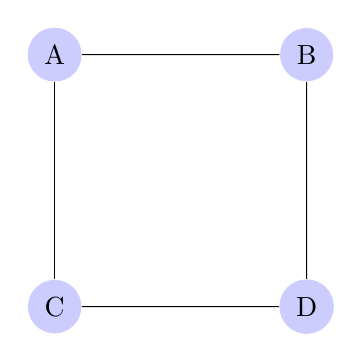
\begin{tikzpicture}
  [scale=.8,auto=left,every node/.style={circle,fill=blue!20}]
  \node (n1) at (1,5) {A};
  \node (n2) at (5,5) {B};
  \node (n3) at (1,1) {C};
  \node (n4) at (5,1) {D}; 


  \foreach \from/\to in {n1/n2,n1/n3,n3/n4,n2/n4}
    \draw (\from) -- (\to);

\end{tikzpicture}
\end{center}
Find a formula for the number of walks of length $k$ from vertex $A$ to vertex $B$, and prove that your answer is correct.
\end{problem}



\begin{problem}
Prove that in any graph the sum of the degrees of all the vertices is even. Deduce that an even number of vertices have odd degree.

\

If I am at a party and have shaken hands with 5 people prove that someone else at the party has shaken hands with an odd number of people.
\end{problem}

\begin{problem}
Is it possible for a graph with an even number of vertices to have half its vertices of degree $a$ and half its vertices of degree $a+1$? If it is then find and prove a necessary condition on the number of vertices and then give an example that is both simple and connected. If it is not then prove that no such graph exists.
\end{problem}

\begin{problem}
A simple graph that is isomorphic to its complement is \emph{self-complementary}. Prove that if $G$ is self-complementary then $G$ has $4k$ or $4k+1$ vertices, where $k$ is an integer. 

\


Find a connected self-complementary graph with 8 vertices.
\end{problem}



\begin{problem}
Prove that no simple graph with 2 or 3 vertices is self-complementary without using Q4.
\end{problem}



\begin{problem}
For each of the following graphs find the degrees of the vertices. Deduce that although all have the same number of vertices and edges, only \emph{exactly} one pair of them is isomorphic. Find an isomorphism between them.
$$\includegraphics[scale=1.5]{2019figs/sixiso.pdf}$$
\end{problem}



\begin{problem}
Let $Q_k$ be the graph whose vertices correspond to the sequences $(a_1, a_2, \ldots , a_k)$ where each $a_i = 0$ or $1$, and whose edges join those sequences that differ in just one place e.g.  $Q_3$ is shown below.
$$\includegraphics[scale=0.75]{2019figs/Q3.pdf}$$
\end{problem}

Find and prove a formula for the number of vertices of $Q_k$. Find and prove a formula for the number of edges of $Q_k$. 


\end{document}